\section{Worked exercise}

We solve now the flow problem summarized in Fig.~\ref{enu01}. We want
to reproduce the water flow in an isotropic soil with a thickness of
9.2 meters, which is formed by silty sand with permeability
coefficient ($k_x=k_y=k_z=5\cdot 10^{-5}$ m / s) and borders on its
bottom edge with a layer of impermeable clay. In this sandy stratum a
sheet pile of 4.6 m.~height and an assumed infinite length (in the
direction perpendicular to the plane of the drawing) has been
nailed. To the left of the sheet piling (upstream) a height of 3
meters of water has accumulated and to the right (downstream) the
runoff makes no accumulation of water. For the problem thus defined
and assuming a stationary regime:
\begin{enumerate}
\item Obtain the outflow water flow downstream (per unit length in the
  $y$ direction).
\item Obtain the evolution of the total head of the fluid
  in the BCD path and estimate the value of the hydraulic gradient at
  point D.
\end{enumerate}

\begin{figure}[!h]
  \begin{center}
    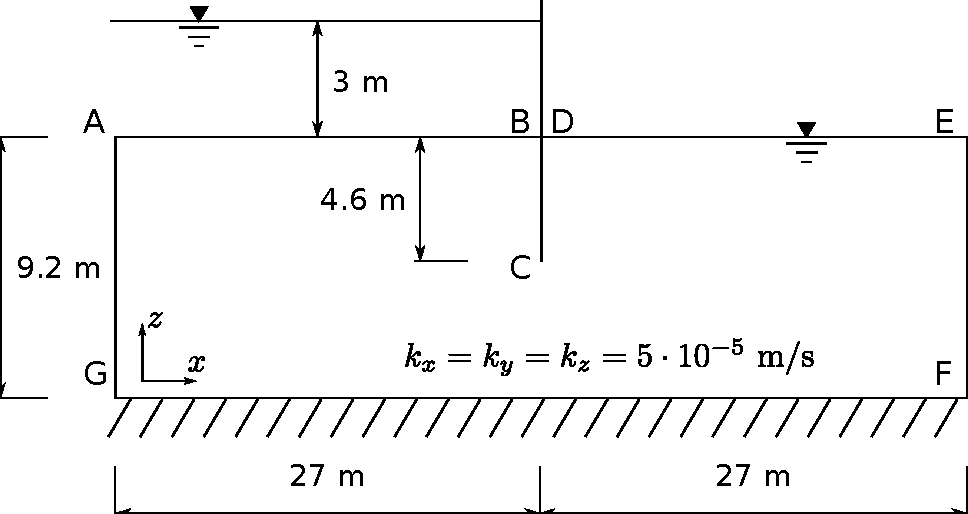
\includegraphics[width=0.75\textwidth]{./body/images/enu01}
  \end{center}
  \caption{Model description}
  \label{enu01}
\end{figure}

The units we are going to use are summarized in Table \ref{tab:201}:
\begin{table}[!h]
  \centering
  \begin{tabular}{lc}
    \hline
    Magnitude&Units\\
    \hline
    Length & m\\
    Total Fluid Head $h$ & m \\
    Coefficient of permeability $k$ & m/s\\
    Flow vector $\mathbf{q}$ & m$^3$/s/m$^2$ \\
    Hydraulic gradient $\mathbf{i}_h$ & m/m \\
    \hline
  \end{tabular}
  \caption{Units}
  \label{tab:201}
\end{table}

To solve this problem we start Abaqus as in previous practice 1 and
define a work directory called \textit{Practica02}. In the remaining
of this section we describe the needed actions to be made in each of
the Abaqus modules to perform the analysis.

\subsection{Module Part. Create the geometry of the elements}
We activate the \textit{Part} module (see Fig.~\ref{part01}) and
create a new object \textbf{2D Planar}, \textbf{Deformable} and
\textbf{Shell} (see Fig.~\ref{part02}).
\begin{figure}[!h]
  \centering
  \begin{subfigure}[!h]{0.29\textwidth}
    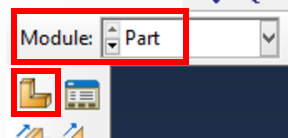
\includegraphics[width=\textwidth]{./body/images/part01.pdf}
    \caption{Start \textbf{Part} module}
    \label{part01}
  \end{subfigure}%
  ~ %add desired spacing between images, e. g. ~, \quad, \qquad, \hfill etc.
  % (or a blank line to force the subfigure onto a new line)
  \begin{subfigure}[!h]{0.39\textwidth}
    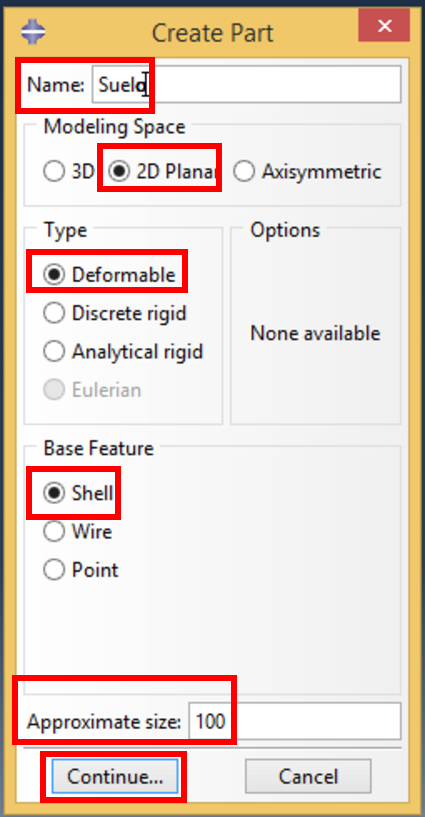
\includegraphics[width=\textwidth]{./body/images/part02.pdf}
    \caption{\textbf{Create Part} dialog box}
    \label{part02}
  \end{subfigure}%
  \caption{Start \textbf{Part} module and \textbf{Create Part} dialog
    box}
\end{figure}

With the \textit{Sketcher} tool, we define the geometry of the problem
as shown in Fig.~\ref{part03}, finally obtaining the new \textit{part}
shown in Fig.~\ref{part04}.
\begin{figure}[!h]
  \centering
  \begin{subfigure}[!h]{1.0\textwidth}
    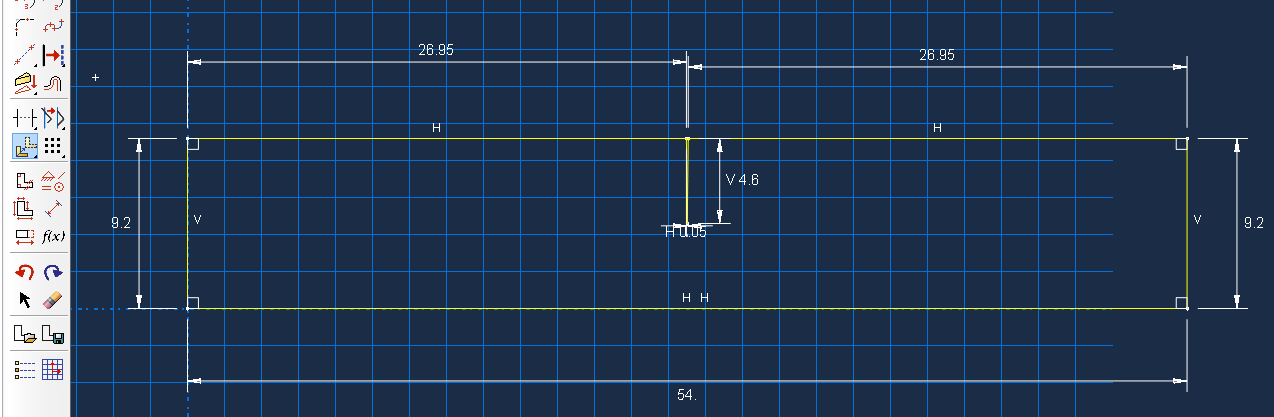
\includegraphics[width=\textwidth]{./body/images/part03}
    \caption{Definition of geometry}
    \label{part03}
  \end{subfigure}%
    
  % add desired spacing between images, e. g. ~, \quad, \qquad,
  % \hfill etc.
  % (or a blank line to force the subfigure onto a new line)
  \begin{subfigure}[!h]{0.875\textwidth}
    
\includegraphics[width=\textwidth]{./body/images/part04}
    \caption{New \textbf{Part}}
    \label{part04}
  \end{subfigure}%
  \caption{Construction of a new \textbf{Part}}
\end{figure}

\subsection{Module Property. Define materials and sections}

We now activate the \textbf{Property} module and define a new material
\textbf{Thermal}, \textbf{Isotropic} and with a conductivity of
$5\cdot 10^{-5}$ as shown in Figs.~\ref{prop01} to \ref{prop03}.
\begin{figure}[!h]
  \centering
  \begin{subfigure}[!h]{0.22\textwidth}
    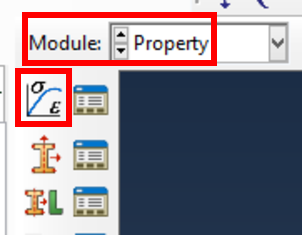
\includegraphics[width=\textwidth]{./body/images/prop01.pdf}
    \caption{Command \textbf{Create Material}}
    \label{prop01}
  \end{subfigure}%
  ~ %add desired spacing between images, e. g. ~, \quad, \qquad, \hfill etc.
  % (or a blank line to force the subfigure onto a new line)
  \begin{subfigure}[!h]{0.36\textwidth}
    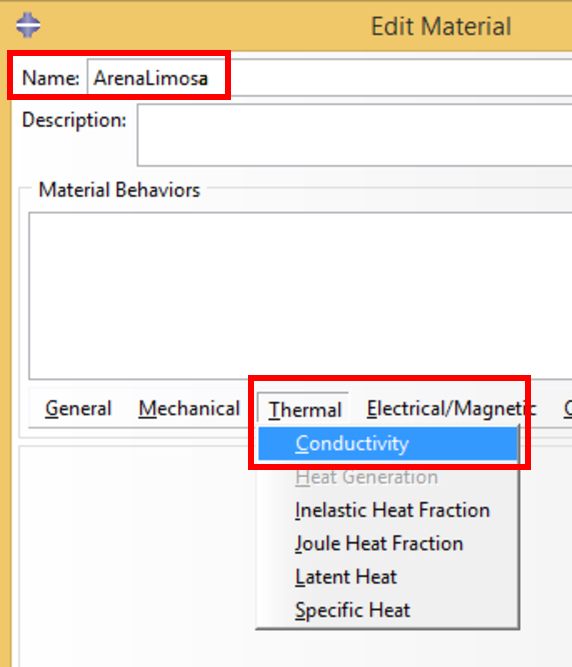
\includegraphics[width=\textwidth]{./body/images/prop02.pdf}
    \caption{Behaviour selection}
    \label{prop02}
  \end{subfigure}%
  ~
  \begin{subfigure}[!h]{0.36\textwidth}
    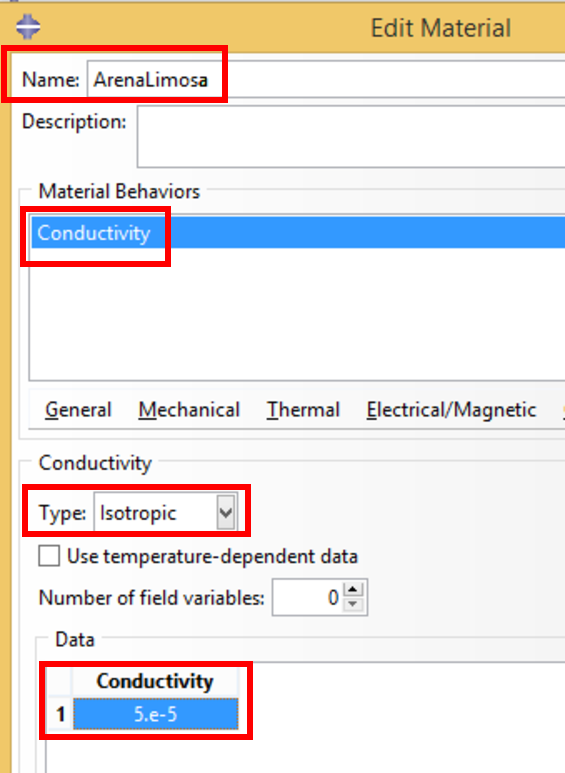
\includegraphics[width=\textwidth]{./body/images/prop03.pdf}
    \caption{Material parameter definition}
    \label{prop03}
  \end{subfigure}%
  \caption{Definition of a new material}
\end{figure}

Once the material has been defined, we must create a new section of
\textbf{Solid} and \textbf{Homogeneous} type following the steps of
Figs.~\ref{prop03p} to \ref{prop05}.
\begin{figure}[!h]
  \centering
  \begin{subfigure}[!h]{0.20\textwidth}
    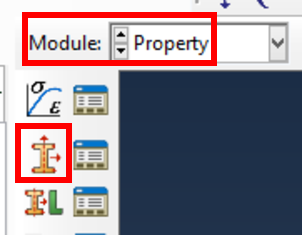
\includegraphics[width=\textwidth]{./body/images/prop03p.pdf}
    \caption{Command \textbf{Create Section}}
    \label{prop03p}
  \end{subfigure}%
  ~
  \begin{subfigure}[!h]{0.39\textwidth}
    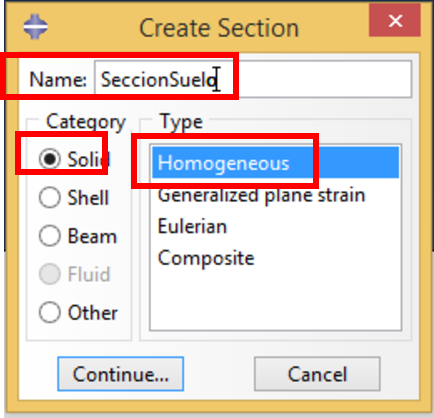
\includegraphics[width=\textwidth]{./body/images/prop04.pdf}
    \caption{Defining the properties of the section}
    \label{prop04}
  \end{subfigure}%
  ~ %add desired spacing between images, e. g. ~, \quad, \qquad, \hfill etc.
  % (or a blank line to force the subfigure onto a new line)
  \begin{subfigure}[!h]{0.39\textwidth}
    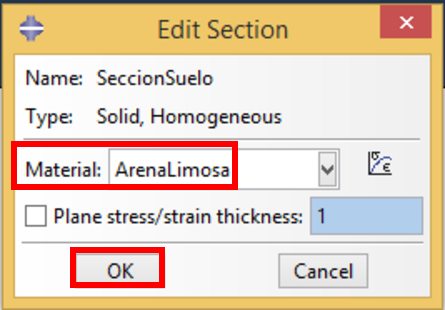
\includegraphics[width=\textwidth]{./body/images/prop05.pdf}
    \caption{Allocation of the material to the section}
    \label{prop05}
  \end{subfigure}%
  \caption{Definition of section \textit{SeccionSuelo}}
\end{figure}

Finally we assign the created section to the \textbf{part} as
summarized in Figs.~\ref{prop05p} to \ref{prop07}.

  \begin{figure}[!h]
    \centering
    \begin{subfigure}[!h]{0.20\textwidth}
      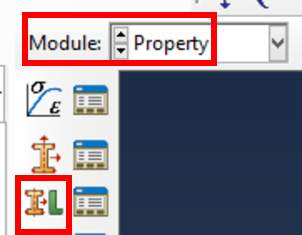
\includegraphics[width=\textwidth]{./body/images/prop05p.pdf}
      \caption{Command \textbf{Assign Section}}
      \label{prop05p}
    \end{subfigure}%
    ~
    \begin{subfigure}[!h]{0.39\textwidth}
      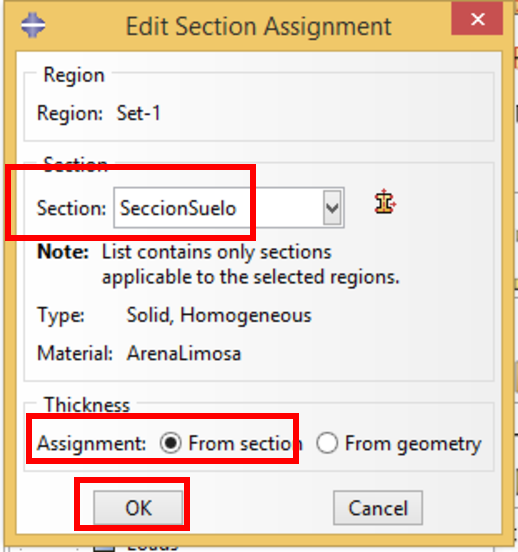
\includegraphics[width=\textwidth]{./body/images/prop06.pdf}
      \caption{Linking the section to a \textit{Part}}
      \label{prop06}
    \end{subfigure}%
    
    % add desired spacing between images, e. g. ~, \quad, \qquad,
    % \hfill etc.
    % (or a blank line to force the subfigure onto a new line)
    \begin{subfigure}[!h]{0.75\textwidth}
      
\includegraphics[width=\textwidth]{./body/images/prop07.png}
      \caption{\textit{Part} with assigned section}
      \label{prop07}
    \end{subfigure}%
    \caption{Assigning the section to a \textbf{Part}}
  \end{figure}

  \subsection{Module Assembly. Assemble the model}

  In the \textit{Assembly} module we assemble our model by making a
  dependent copy of our part as shown in Figs.~\ref{asse01} and
  \ref{asse02}.
  \begin{figure}[!h]
    \centering
    \begin{subfigure}[!h]{0.25\textwidth}
      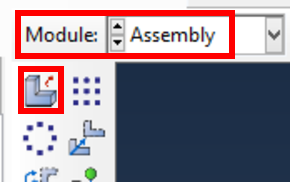
\includegraphics[width=\textwidth]{./body/images/asse01.pdf}
      \caption{Command \textbf{Create Instance}}
      \label{asse01}
    \end{subfigure}%
    ~ %add desired spacing between images, e. g. ~, \quad, \qquad, \hfill etc.
    % (or a blank line to force the subfigure onto a new line)
    \begin{subfigure}[!h]{0.39\textwidth}
      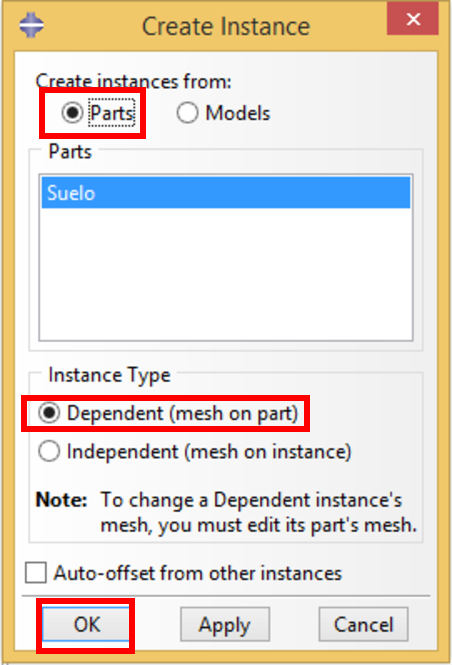
\includegraphics[width=\textwidth]{./body/images/asse02.pdf}
      \caption{Creation of a \textbf{Dependent} instance}
      \label{asse02}
    \end{subfigure}%
    \caption{\textbf{Create Instance}}
  \end{figure}

  \subsection{Module Step. Configure the analysis procedure}

  We need to create a calculation step (\textbf{Heat Transfer} type)
  with the option \textbf{Steady-state} (see Figs.~\ref{step01} to
  \ref{step03}) .
  \begin{figure}[!h]
    \centering
    \begin{subfigure}[!h]{0.20\textwidth}
      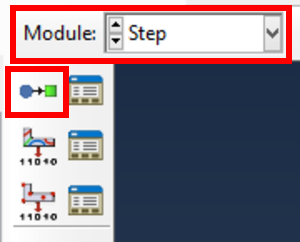
\includegraphics[width=\textwidth]{./body/images/step01.pdf}
      \caption{Command \textbf{Create Step}}
      \label{step01}
    \end{subfigure}%
    ~
    \begin{subfigure}[!h]{0.39\textwidth}
      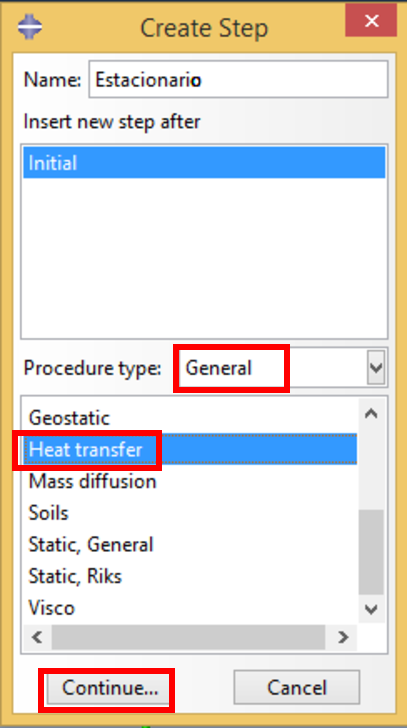
\includegraphics[width=\textwidth]{./body/images/step02.pdf}
      \caption{Properties of new step}
      \label{step02}
    \end{subfigure}%
    ~ %add desired spacing between images, e. g. ~, \quad, \qquad, \hfill etc.
    % (or a blank line to force the subfigure onto a new line)
    \begin{subfigure}[!h]{0.39\textwidth}
      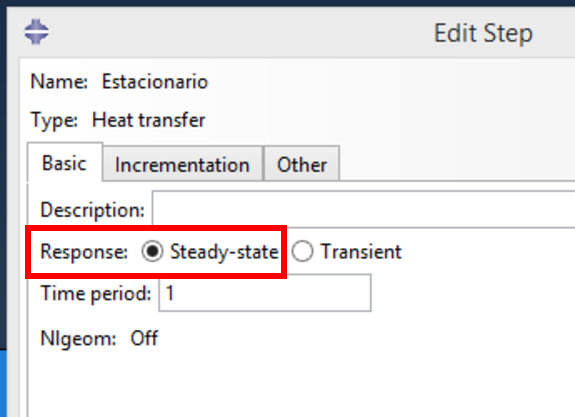
\includegraphics[width=\textwidth]{./body/images/step03.pdf}
      \caption{Steady-state selection}
      \label{step03}
    \end{subfigure}%
    \caption{Creating a new calculation step}
  \end{figure}

  As we have defined a steady state regime, Abaqus does not generate a
  \textbf{History Output}. Let's review the data we are going to save
  for the post-processing by opening the \textbf{Field Output} that
  Abaqus creates by default, and making sure that we store
  the \textbf{Nodal temperatures}, the \textbf{Heat flux vector} and
  the \textbf{Reaction fluxes} (fluxes calculated where we apply a temperature
  Dirchlet-type boundary condition) as indicated in Figs.~\ref{step04}
  and \ref{step05}.
  \begin{figure}[!h]
    \centering
    \begin{subfigure}[!h]{0.45\textwidth}
      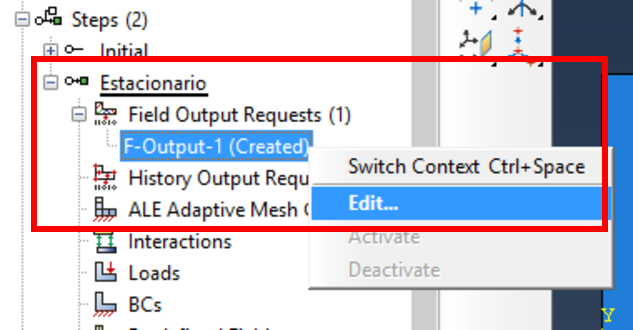
\includegraphics[width=\textwidth]{./body/images/step04.pdf}
      \caption{\textbf{Field Output} selection}
      \label{step04}
    \end{subfigure}%
    ~ %add desired spacing between images, e. g. ~, \quad, \qquad, \hfill etc.
    % (or a blank line to force the subfigure onto a new line)
    \begin{subfigure}[!h]{0.45\textwidth}
      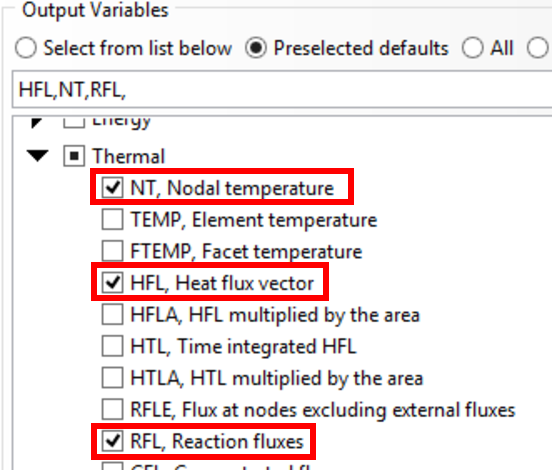
\includegraphics[width=\textwidth]{./body/images/step05.pdf}
      \caption{Post-process values to be saved}
      \label{step05}
    \end{subfigure}%
    \caption{\textit{Field Output} definition}
  \end{figure}

  \subsection{Module Load. Apply the boundary conditions}

  In the case of confined flow problems we can find the following two
  boundary conditions (in our problem we will impose a constant value
  to the boundary conditions because we assume we are in a steady
  state):
  \begin{description}
  \item[Essential-type] Boundaries where we impose the value of the
    total head of the fluid $h=h^*$.
  \item[Natural-type] Boundaries where we impose the value of the flux
    $(-\textbf{k}\cdot\bm{\nabla}h)\cdot\textbf{n}=\mathrm{cte}$,
    being $\textbf{n}$ the normal outside the boundary where we impose
    the value of the flow.
  \end{description}

  If we impose nothing on an boundary of our domain, Abaqus
  understands that we are imposing a null flow across that border
  (impermeable border), which means that we are imposing
  $ \bm{\nabla}h\cdot\textbf{n}=0$.

  In our case we have to impose:
  \begin{enumerate}
  \item Two essential boundary conditions at the top of the domain
    (assuming the datum is on the horizontal line AE).
    \begin{itemize}
    \item $h=u_A/\gamma_w+z_A=\dfrac{\rho_w\; g\; 3}{\rho_w g}+0 = 3$
      m in the equipotential AB.
    \item $h=u_E/\gamma_w+z_E= \dfrac{\rho_w\; g\; 0}{\rho_w g}+0=0$ m
      in the equipotential DE
    \end{itemize}
    We will impose these conditions in the created step called
    \textit{estacionario}.
  \item The natural-type boundary condition ``impermeable boundary''
    $\bm{\nabla}h \cdot \textbf{n} = 0 $ in the AGFE and BCD
    boundaries. This boundary condition is kept fixed throughout the
    analysis and we could define it in the step \textit{Initial}
    created by Abaqus to be propagated to the rest of steps. However,
    since this condition (impermeable border) is defined by default,
    it is not necessary for us to define anything.
  \end{enumerate}

  To impose the essential boundary condition $h=3$ in the boundary
  $AB$, we activate the \textbf{Load} module and press the
  \textbf{Create Boundary Condition} command (see
  Fig.~\ref{load02}). Then follow the instructions given in
  Figs.~\ref{load03} to \ref{load05}.

  \begin{figure}[!h]
    \centering
    \begin{subfigure}[!h]{0.25\textwidth}
      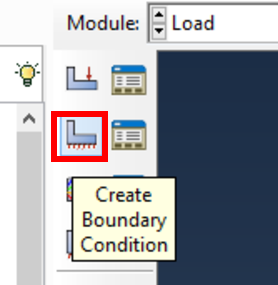
\includegraphics[width=\textwidth]{./body/images/load02.pdf}
      \caption{Command \textbf{Create Boundary Condition}}
      \label{load02}
    \end{subfigure}%
    ~ %add desired spacing between images, e. g. ~, \quad, \qquad, \hfill etc.
    % (or a blank line to force the subfigure onto a new line)
    \begin{subfigure}[!h]{0.45\textwidth}
      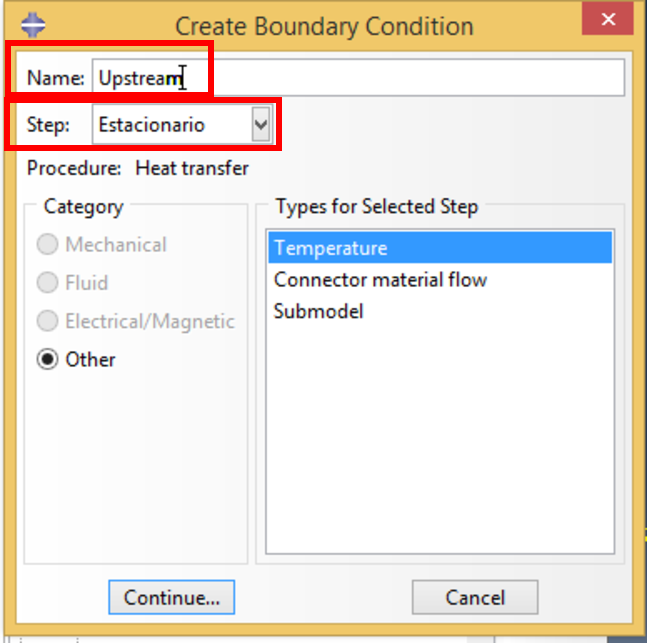
\includegraphics[width=\textwidth]{./body/images/load03.pdf}
      \caption{Definition of essential-type boundary condition}
      \label{load03}
    \end{subfigure}%

    \begin{subfigure}[!h]{0.52\textwidth}
      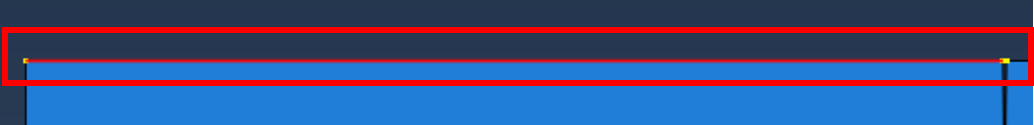
\includegraphics[width=\textwidth]{./body/images/load04.pdf}
      \caption{Boundary selection}
      \label{load04}
    \end{subfigure}%
    ~ %add desired spacing between images, e. g. ~, \quad, \qquad, \hfill etc.
    % (or a blank line to force the subfigure onto a new line)
    \begin{subfigure}[!h]{0.45\textwidth}
      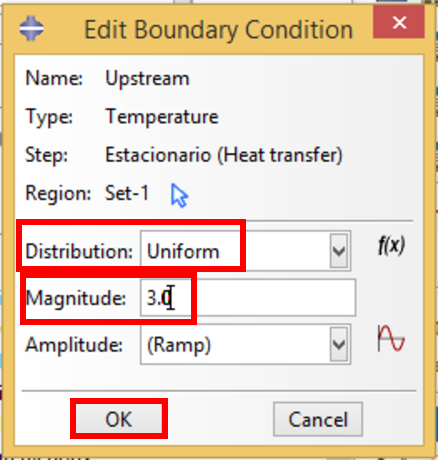
\includegraphics[width=\textwidth]{./body/images/load05.pdf}
      \caption{Definition of imposed total head}
      \label{load05}
    \end{subfigure}%
    \caption{Definition of the boundary condition in the equipotential
      AB}
  \end{figure}

  Likewise, to impose the essential-type boundary conditions $h=0$ in
  the boundary DE follows the instructions given in Figs.~\ref{load06}
  to \ref{load08}. At the end Abaqus indicates the boundaries where
  you have imposed boundary conditions as shown in Fig.~\ref{load09}.

  \begin{figure}[!h]
    \centering
    \begin{subfigure}[!h]{0.42\textwidth}
      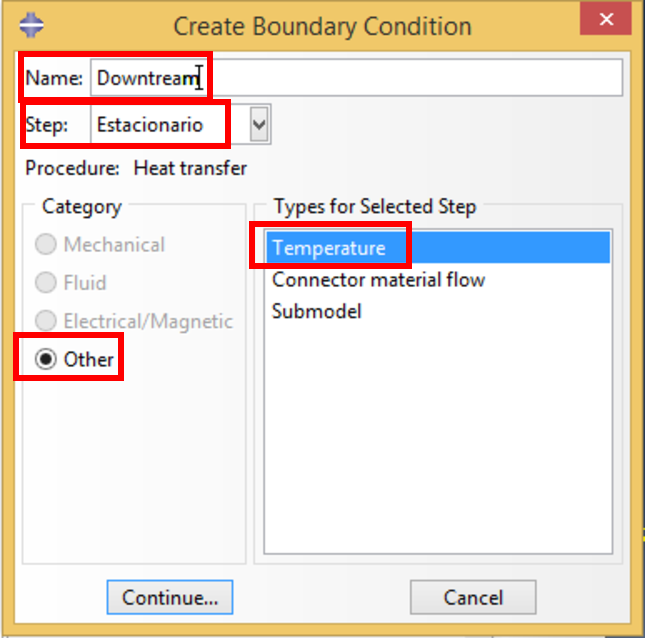
\includegraphics[width=\textwidth]{./body/images/load06.pdf}
      \caption{Definition of essential-type boundary condition}
      \label{load06}
    \end{subfigure}%
    ~ %add desired spacing between images, e. g. ~, \quad, \qquad, \hfill etc.
    % (or a blank line to force the subfigure onto a new line)
    \begin{subfigure}[!h]{0.55\textwidth}
      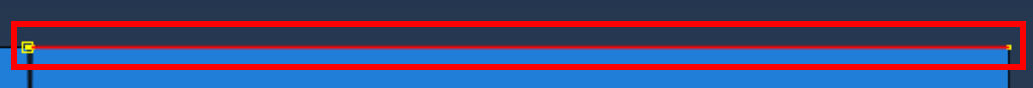
\includegraphics[width=\textwidth]{./body/images/load07.pdf}
      \caption{Boundary selection}
      \label{load07}
    \end{subfigure}%

    \begin{subfigure}[!h]{0.42\textwidth}
      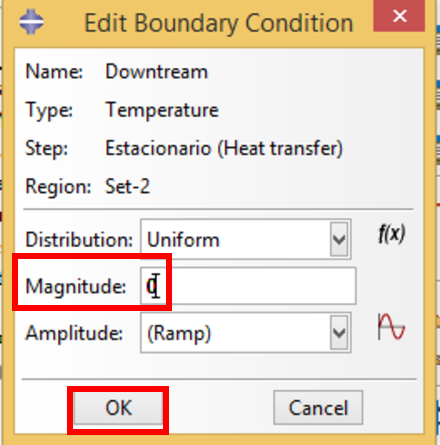
\includegraphics[width=\textwidth]{./body/images/load08.pdf}
      \caption{Definition of imposed total head}
      \label{load08}
    \end{subfigure}%
    ~ %add desired spacing between images, e. g. ~, \quad, \qquad, \hfill etc.
    % (or a blank line to force the subfigure onto a new line)
    \begin{subfigure}[!h]{0.55\textwidth}
      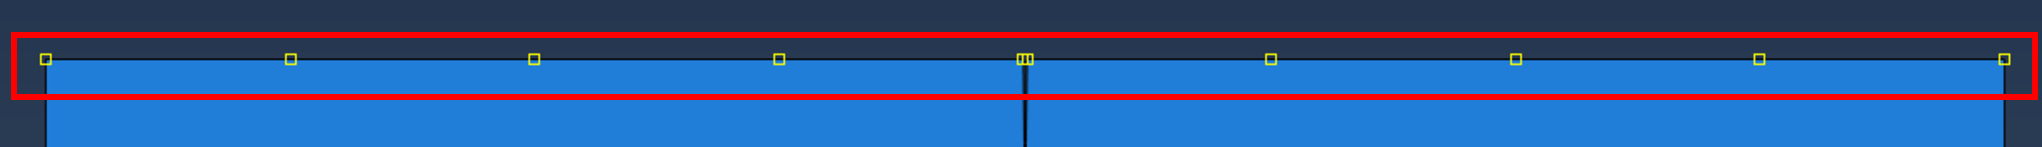
\includegraphics[width=\textwidth]{./body/images/load09.pdf}
      \caption{Definition of imposed total head}
      \label{load09}
    \end{subfigure}%
    \caption{Definition of the boundary condition in the equipotential
      DE}
  \end{figure}


  \subsection{Module Mesh. Create the mesh.}

  In order to build the mesh, let's remember the actions we studied
  in previous practice 1:
  \begin{enumerate}
  \item Activate the \textbf{Mesh} module and, since we have assembled
    the model with a dependent copy, we impose that we will mesh the
    \textbf {part} as indicated in Fig.~\ref{mess01}.
    \begin{figure}[!h]
      \begin{center}
        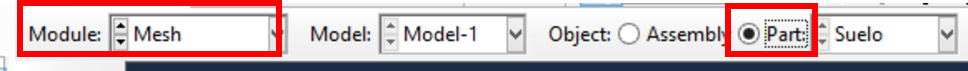
\includegraphics[width=0.9\textwidth]{./body/images/mess01.pdf}
      \end{center}
      \caption{Start \textbf{mesh} module}
      \label{mess01}
    \end{figure}
  \item Define the element shape (quadrilaterals) (see
    Fig.~\ref{mess02}).
    \begin{figure}[!h]
      \begin{center}
        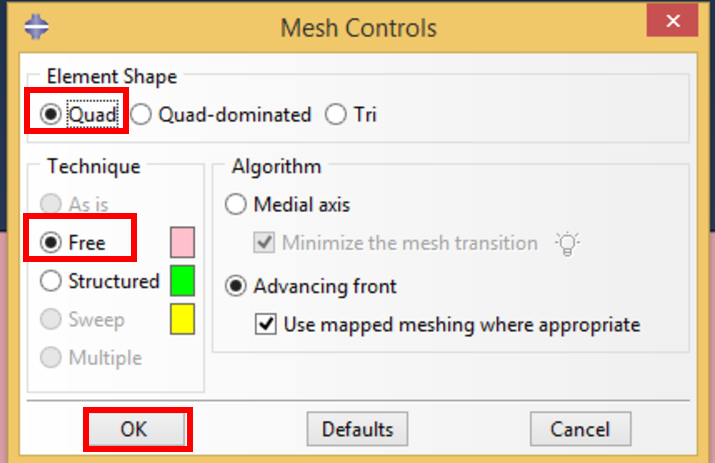
\includegraphics[width=0.45\textwidth]{./body/images/mess02.pdf}
      \end{center}
      \caption{Shape element definition}
      \label{mess02}
    \end{figure}
  \item Set the global size of the element to 1.5 meters (see
    Fig.~\ref{mess03})
    \begin{figure}[!h]
      \begin{center}
        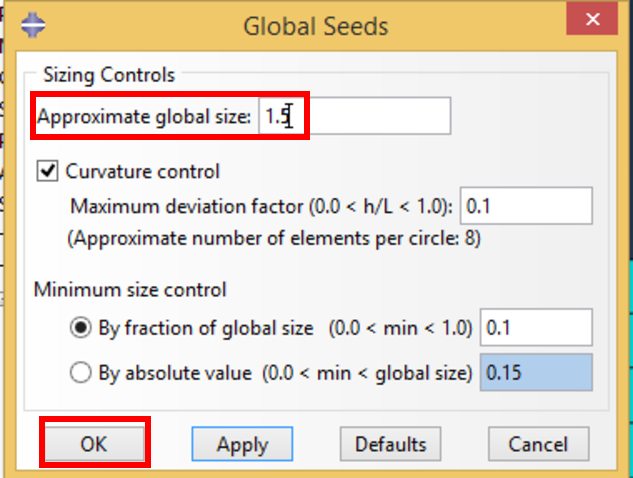
\includegraphics[width=0.45\textwidth]{./body/images/mess03.pdf}
      \end{center}
      \caption{Element size definition}
      \label{mess03}
    \end{figure}
  \item Finally we define the type of interpolation as indicated in Fig.~\ref{mess04}.
    \begin{figure}[!h]
      \begin{center}
        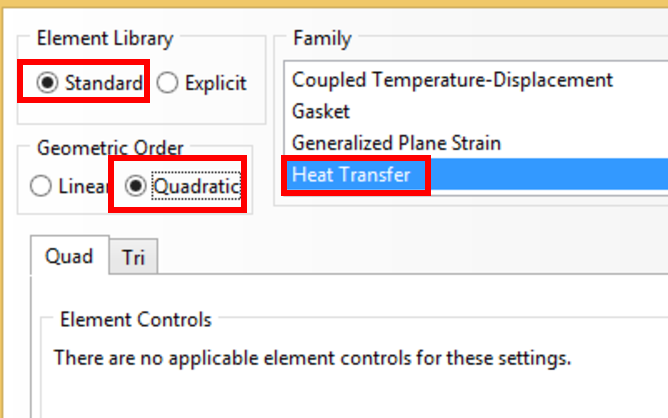
\includegraphics[width=0.45\textwidth]{./body/images/mess04.pdf}
      \end{center}
      \caption{Type of element definition}
      \label{mess04}
    \end{figure}
  \end{enumerate}

  Final mesh is shown in Fig.~\ref{mess05}.
  \begin{figure}[!h]
    \begin{center}
      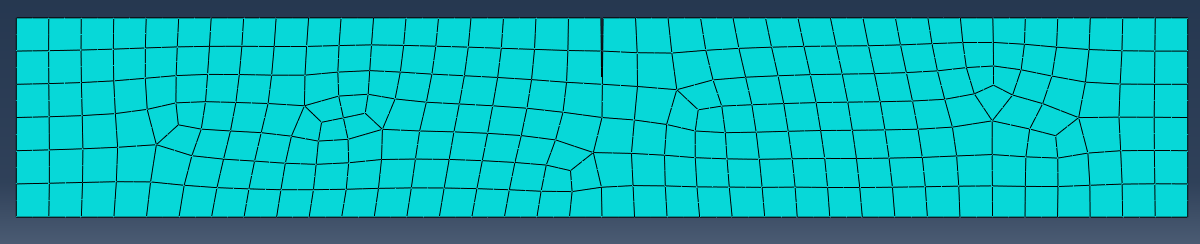
\includegraphics[width=0.85\textwidth]{./body/images/mess05}
    \end{center}
    \caption{Final mesh}
    \label{mess05}
  \end{figure}

  \subsection{Module Job. Create the job and run the analysis.}

  Once we have defined the model we only need to create and launch the
  \textbf{job}. To do this activate the \textbf{job} module,
  click on the \textbf {Create job} icon (see Fig.~\ref{job01}) and
  follow the instructions in Figs.~\ref{job02} and \ref{job03}.
  \begin{figure}[!h]
    \centering
    \begin{subfigure}[!h]{0.21\textwidth}
      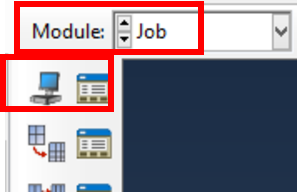
\includegraphics[width=\textwidth]{./body/images/job01.pdf}
      \caption{Command \textbf{Create Job}}
      \label{job01}
    \end{subfigure}%
    ~ %add desired spacing between images, e. g. ~, \quad, \qquad, \hfill etc.
    % (or a blank line to force the subfigure onto a new line)
    \begin{subfigure}[!h]{0.32\textwidth}
      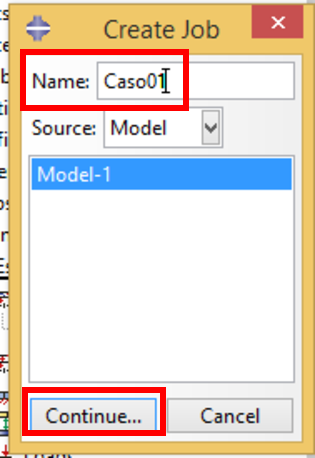
\includegraphics[width=\textwidth]{./body/images/job02.pdf}
      \caption{\textit{Create Job} dialog box}
      \label{job02}
    \end{subfigure}%
    ~
    \begin{subfigure}[!h]{0.44\textwidth}
      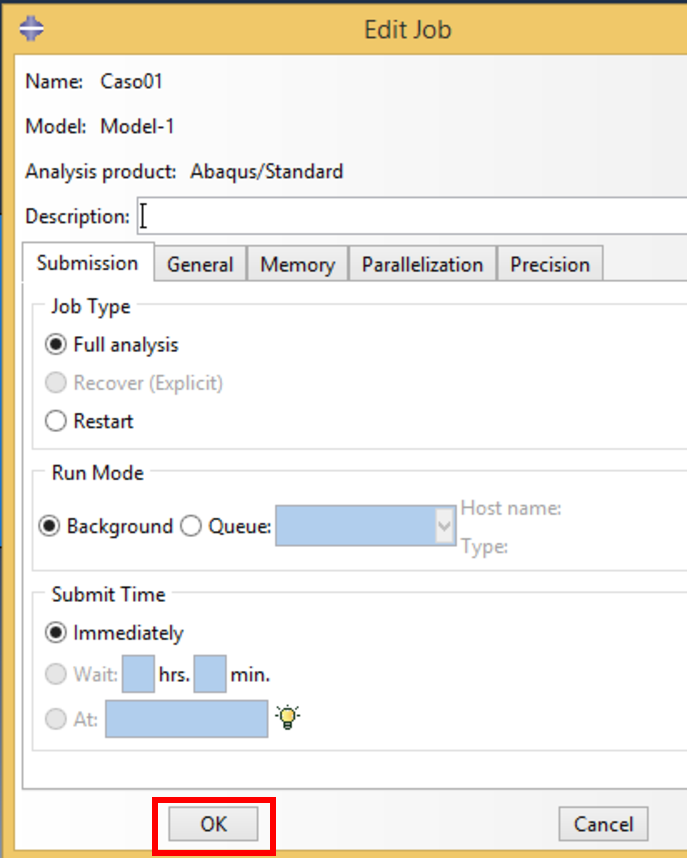
\includegraphics[width=\textwidth]{./body/images/job03.pdf}
      \caption{Parameters of the analysis}
      \label{job03}
    \end{subfigure}%
    \caption{Job definition}
  \end{figure}

  Finally launch the job and, once the numerical analysis converges,
  activate the post process (see Figs.~\ref{job04} and \ref{job05}).
  \begin{figure}[!h]
    \centering
    \begin{subfigure}[!h]{0.42\textwidth}
      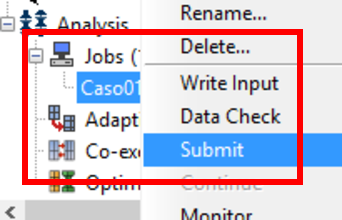
\includegraphics[width=\textwidth]{./body/images/job04.pdf}
      \caption{Job submission}
      \label{job04}
    \end{subfigure}%
    ~ %add desired spacing between images, e. g. ~, \quad, \qquad, \hfill etc.
    % (or a blank line to force the subfigure onto a new line)
    \begin{subfigure}[!h]{0.42\textwidth}
      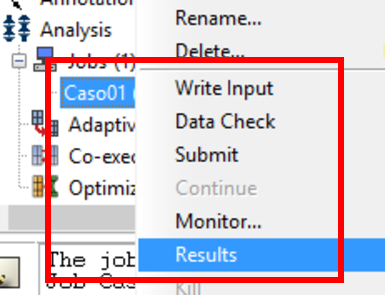
\includegraphics[width=\textwidth]{./body/images/job05.pdf}
      \caption{Post-process activation}
      \label{job05}
    \end{subfigure}%
    \caption{Job launch}
  \end{figure}

  \subsection{Module Visualization. Post-process.}
  Next, the needed post process actions are summarized in order to
  answer the questions of the exercise:
  \begin{itemize}
  \item Let us first draw the field of the total head of the fluid at
    each point (see Figs.~\ref{post01} and \ref{post02}). If we would
    like to obtain the equipotential lines, we activate the
    \textbf{Contour Plot Options} command and set that the type of
    contour is \textbf{line} as indicated by Figs.~\ref{post03} and
    \ref{post04}.
    \begin{figure}[!h]
      \centering
      \begin{subfigure}[!h]{0.21\textwidth}
        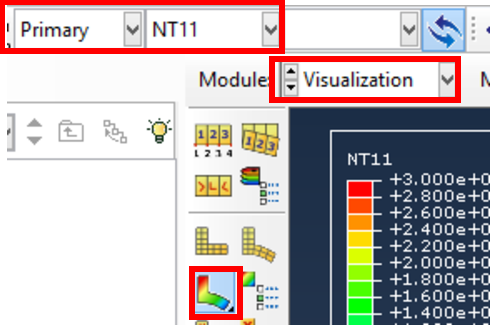
\includegraphics[width=\textwidth]{./body/images/post01.pdf}
        \caption{Command \textbf{Plot Contours on deformed shape}}
        \label{post01}
      \end{subfigure}%
      ~ %add desired spacing between images, e. g. ~, \quad, \qquad, \hfill etc.
      % (or a blank line to force the subfigure onto a new line)
      \begin{subfigure}[!h]{0.60\textwidth}
        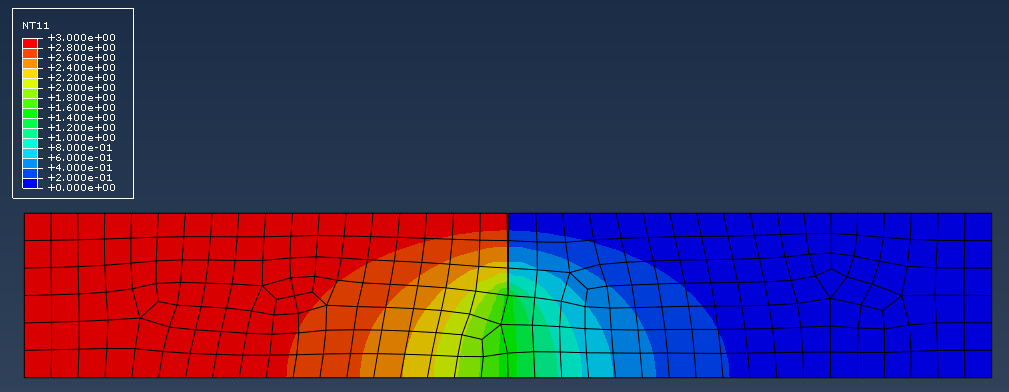
\includegraphics[width=\textwidth]{./body/images/post02}
        \caption{Distribution of total fluid head}
        \label{post02}
      \end{subfigure}%

      \begin{subfigure}[!h]{0.40\textwidth}
        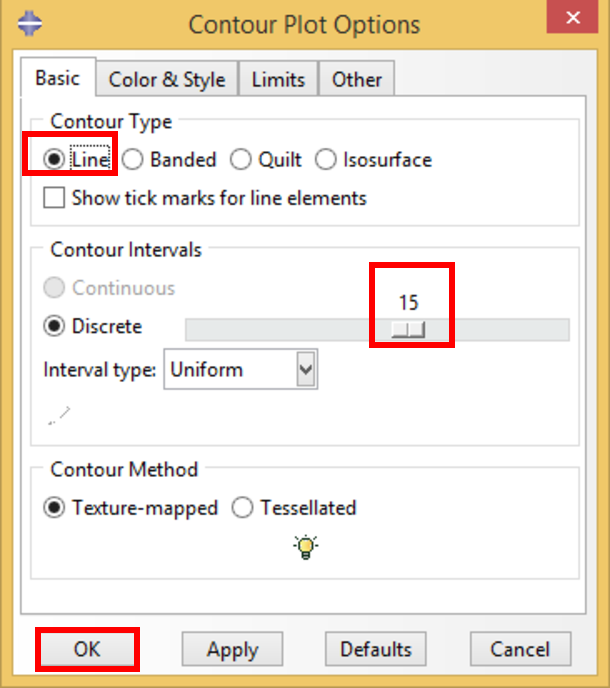
\includegraphics[width=\textwidth]{./body/images/post03.pdf}
        \caption{\textbf{Contour Plots} dialog box}
        \label{post03}
      \end{subfigure}%
      \begin{subfigure}[!h]{0.60\textwidth}
        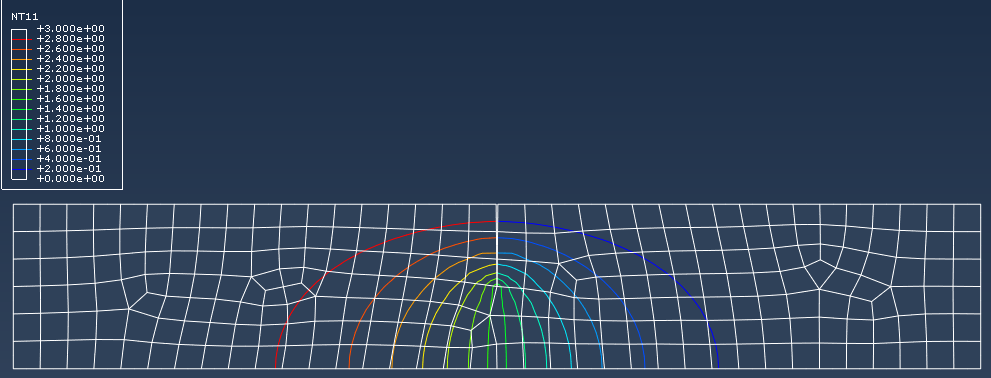
\includegraphics[width=\textwidth]{./body/images/post04}
        \caption{Distribution of total fluid head (equipotentials)}
        \label{post04}
      \end{subfigure}%
      \caption{Display of total fluid head}
    \end{figure}

  \item We want to answer now the first of the exercise questions, to
    obtain the outflow downstream. To do so we must obtain the
    distribution of the outflow in the line DE and integrate it. Let
    us first define a \textbf{path} in the contour DE that we will
    call \textit{CorrienteAbajo} as shown in Figs.~\ref{post05} to
    \ref{post10}.

  \begin{figure}[!h]
    \centering
    \begin{subfigure}[!h]{0.20\textwidth}
      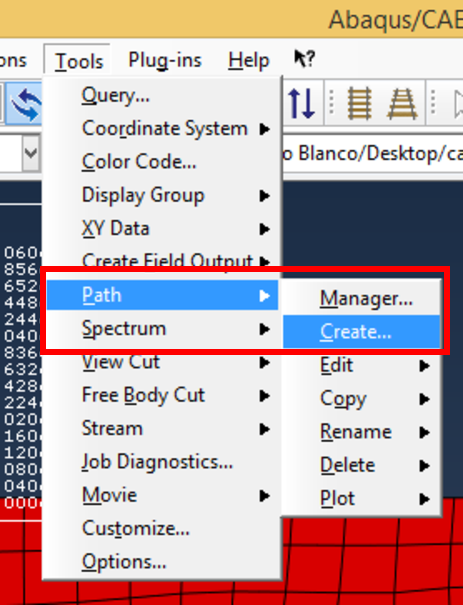
\includegraphics[width=\textwidth]{./body/images/post05.pdf}
      \caption{Command \textbf{Path/Create}}
      \label{post05}
    \end{subfigure}%
    \begin{subfigure}[!h]{0.40\textwidth}
      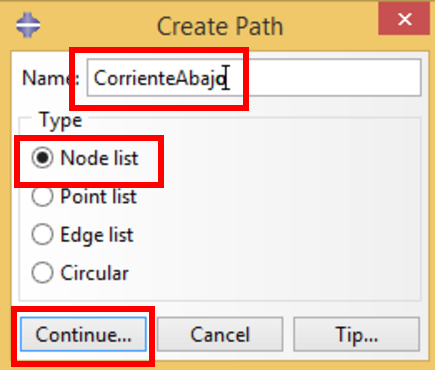
\includegraphics[width=\textwidth]{./body/images/post07.pdf}
      \caption{\textit{Create Path} dialog box}
      \label{post07}
    \end{subfigure}%
    \begin{subfigure}[!h]{0.40\textwidth}
      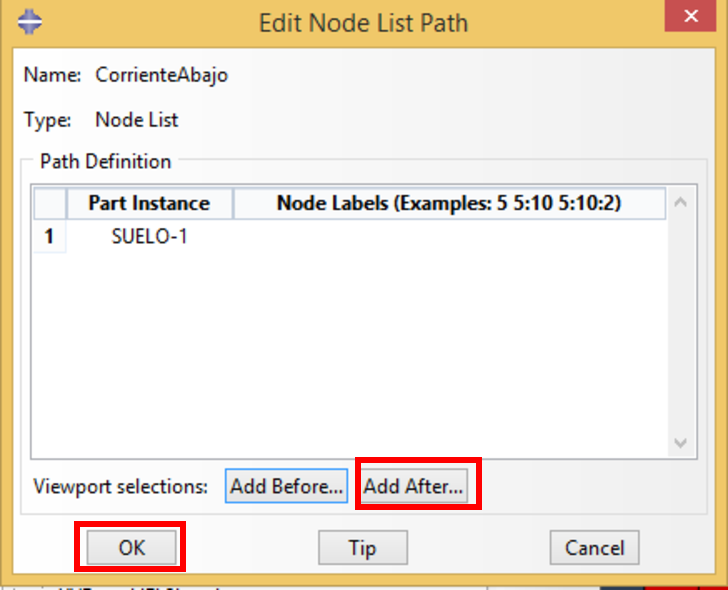
\includegraphics[width=\textwidth]{./body/images/post08.pdf}
      \caption{\textit{Path} geometrical definition}
      \label{post08}
    \end{subfigure}%
    
    \begin{subfigure}[!h]{0.60\textwidth}
      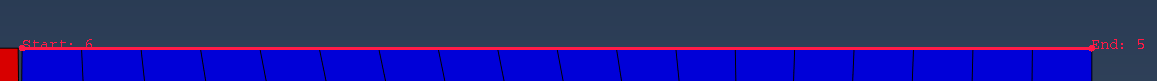
\includegraphics[width=\textwidth]{./body/images/post09}
      \caption{Downstream boundary}
      \label{post09}
    \end{subfigure}%
    \begin{subfigure}[!h]{0.40\textwidth}
      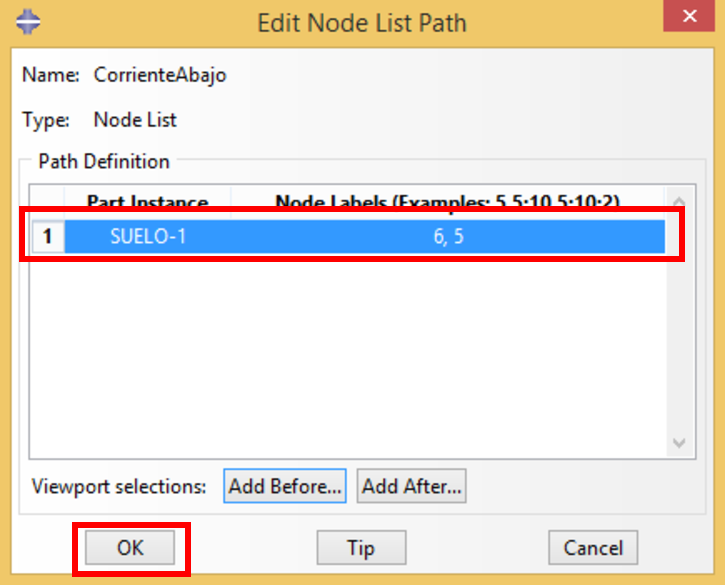
\includegraphics[width=\textwidth]{./body/images/post10.pdf}
      \caption{\textit{path} geometrical definition}
      \label{post10}
    \end{subfigure}%
    \caption{\textit{AguasAbajo} path definition}
  \end{figure}

\item Once the \textit{path} is defined, we look for the distribution
  of the total head along it. To do so we must create an object
  \textbf {XY Data} as summarized in Figs.~\ref{post11} to
  \ref{post15}.
  \begin{figure}[!h]
    \centering
    \begin{subfigure}[!h]{0.21\textwidth}
      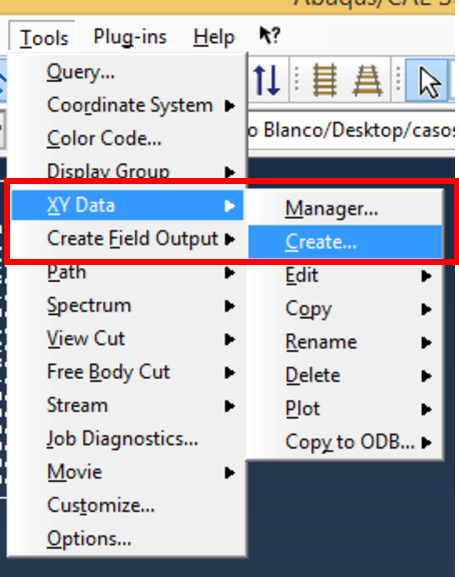
\includegraphics[width=\textwidth]{./body/images/post11.pdf}
      \caption{Command \textbf{XY Data/Create}}
      \label{post11}
    \end{subfigure}%
    \begin{subfigure}[!h]{0.35\textwidth}
      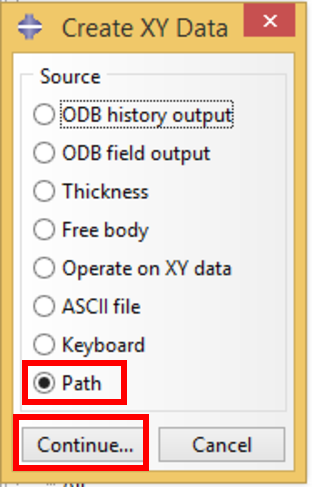
\includegraphics[width=\textwidth]{./body/images/post12.pdf}
      \caption{\textit{XY Data} dialog box}
      \label{post12}
    \end{subfigure}%
    \begin{subfigure}[!h]{0.44\textwidth}
      \includegraphics[width=\textwidth]{./body/images/post13.pdf}
      \caption{\textit{XY Data from path} dialog box}
      \label{post13}
    \end{subfigure}%
    
    \begin{subfigure}[!h]{0.60\textwidth}
      \includegraphics[width=\textwidth]{./body/images/post14.pdf}
      \caption{Selecting the variable to draw in the path}
      \label{post14}
    \end{subfigure}%
    \begin{subfigure}[!h]{0.40\textwidth}
      \includegraphics[width=\textwidth]{./body/images/post15.pdf}
      \caption{\textit{XY Data from path} dialog box}
      \label{post15}
    \end{subfigure}%
    \caption{Definition object XY Data with the total head on the
      boundary DE}
  \end{figure}

\item The distribution of the outflow in the DE boundary is shown in
  Fig.~\ref{post16}. In order to export it to an excel sheet (and
  integrate it) we must save it as shown in Figs.~\ref{post17} and
  \ref{post18}.

  \begin{figure}[!h]
    \centering
    \begin{subfigure}[!h]{0.80\textwidth}
      \includegraphics[width=\textwidth]{./body/images/post16}
      \caption{Distribution of the outflow in straight line DE}
      \label{post16}
    \end{subfigure}%
    
    \begin{subfigure}[!h]{0.30\textwidth}
      \includegraphics[width=\textwidth]{./body/images/post17.pdf}
      \caption{\textit{Save XY Data As} dialog box}
      \label{post17}
    \end{subfigure}\quad
    \begin{subfigure}[!h]{0.30\textwidth}
      \includegraphics[width=\textwidth]{./body/images/post18.pdf}
      \caption{XY Data objects in the \textit{Model Tree}}
      \label{post18}
    \end{subfigure}%
    \caption{ XY Data objects of the outflow in the line DE}
  \end{figure}

\item Next we export the data from the XY Data object we just created
  as indicated by Figs.~\ref{post19} to \ref{post21}.
  \begin{figure}[!h]
    \centering
    \begin{subfigure}[!h]{0.25\textwidth}
      \includegraphics[width=\textwidth]{./body/images/post19.pdf}
      \caption{Command \textbf{Report/XY}}
      \label{post19}
    \end{subfigure}%
    \begin{subfigure}[!h]{0.37\textwidth}
      \includegraphics[width=\textwidth]{./body/images/post20.pdf}
      \caption{\textit{report XY Data} dialog box}
      \label{post20}
    \end{subfigure}%
    \begin{subfigure}[!h]{0.37\textwidth}
      \includegraphics[width=\textwidth]{./body/images/post21.pdf}
      \caption{\textit{Report XY Data} dialog box}
      \label{post21}
    \end{subfigure}%
    \caption{Save in a plain text file the object XY data}
  \end{figure}

\item In Figs.~\ref{post22} to \ref{post25} how to import the text
  file we just saved in Excel is explained. This information is valid
  for Excel2013.
  \begin{figure}[!h]
    \centering
    \begin{subfigure}[!h]{0.50\textwidth}
      \includegraphics[width=\textwidth]{./body/images/post22.pdf}
      \caption{Import data from text file into excel (I)}
      \label{post22}
    \end{subfigure}%
    \begin{subfigure}[!h]{0.50\textwidth}
      \includegraphics[width=\textwidth]{./body/images/post23.pdf}
      \caption{Import data from text file into excel (II)}
      \label{post23}
    \end{subfigure}%

    \begin{subfigure}[!h]{0.50\textwidth}
      \includegraphics[width=\textwidth]{./body/images/post24.pdf}
      \caption{Import data from text file into excel (III)}
      \label{post24}
    \end{subfigure}%
    \begin{subfigure}[!h]{0.50\textwidth}
      \includegraphics[width=\textwidth]{./body/images/post25.pdf}
      \caption{Import data from text file into excel (IV)}
      \label{post25}
    \end{subfigure}%
    \caption{Import data from text file into excel}
  \end{figure}

\item With the imported data, we integrate the curve flow \textit{vs.}
  distance using the trapezoid method, finally obtaining a value of
  the outflow of $7.67\cdot 10^{-5}$ m$^3$/s per meter in the $y$
  direction (see Fig.~\ref{post26}).
  \begin{figure}[!h]
    \begin{center}
      \includegraphics[width=0.99\textwidth]{./body/images/post26}
    \end{center}
    \caption{Integration of the total flow using the trapezoid method}
    \label{post26}
  \end{figure}

  Equivalently (and faster) we can integrate the curve of
  Fig.~\ref{post16} using Abaqus's \texttt{python} console. The
  XY-Data object we have named XYData-HFL2 (see Fig.~\ref{post18}) is
  an object that Abaqus stores and can be accessed and operated with,
  as shown in Fig.~\ref{post26b} (try as an exercise to understand the
  logic of the python code).
  \begin{figure}[!h]
    \begin{center}
      \includegraphics[width=0.99\textwidth]{./body/images/post26b.pdf}
    \end{center}
    \caption{Integration of the total flow using the trapezoid method
      using \texttt{python}}
    \label{post26b}
  \end{figure}

  Finally, there is a third way to integrate this curve using the Abaqus commands themselves, which allows us to operate with previously created \textit{XYData} objects. Press \textit{Tools/XYData/Create}, but instead of creating a new object according to a \textit{path} we will choose the option \textit{Operate on XYData}, as shown in Fig.~\ref{post26c}.
   \begin{figure}[!h]
    \begin{center}
      \includegraphics[width=0.99\textwidth]{./body/images/post26c.pdf}
    \end{center}
    \caption{Selection of tool \textit{Operate on XYData}}
    \label{post26c}
  \end{figure}

  From all possible operations we select the command \textit{integrate(X)} taking as argument the object \textit{XYData} where we have saved the normal flow to the surface as summarized in Fig.~\ref{post26d}.
    \begin{figure}[!h]
    \begin{center}
      \includegraphics[width=0.99\textwidth]{./body/images/post26d.pdf}
    \end{center}
    \caption{Integration of object \textit{XYData}}
    \label{post26d}
  \end{figure}

  Finally we can draw the value of the flow and its integration along the curve as shown in Fig.~\ref{post26e} and access the value of the total flow for the final ordinate as shown in Fig.~\ref{post26f }.
     \begin{figure}[!h]
    \begin{center}
      \includegraphics[width=0.99\textwidth]{./body/images/post26e.pdf}
    \end{center}
    \caption{Variación del flujo y su integración a lo largo del \textit{path}}
    \label{post26e}
  \end{figure}
      \begin{figure}[!h]
    \begin{center}
      \includegraphics[width=0.99\textwidth]{./body/images/post26f.pdf}
    \end{center}
    \caption{Integración del flujo a lo largo del \textit{path}}
    \label{post26f}
  \end{figure}


  
\item In order to answer the second question we need to obtain the
  evolution of the total head of the fluid in the BCD path and to
  estimate the value of the hydraulic gradient in the point
  D. Therefore we must obtain the distribution of the total head in
  the BCD path and estimate its slope at point D. Similar to the
  previous point, first define a \textbf{path} following the BCD path
  as summarized in Figs.~\ref{post27} to \ref{post30}.
  \begin{figure}[!h]
    \centering
    \begin{subfigure}[!h]{0.50\textwidth}
      \includegraphics[width=\textwidth]{./body/images/post27.pdf}
      \caption{\textit{Create Path} dialog box}
      \label{post27}
    \end{subfigure}%
    \begin{subfigure}[!h]{0.50\textwidth}
      \includegraphics[width=\textwidth]{./body/images/post28.pdf}
      \caption{\textit{Path} geometrical definition}
      \label{post28}
    \end{subfigure}%

    \begin{subfigure}[!h]{0.07\textwidth}
      \includegraphics[width=\textwidth]{./body/images/post29}
      \caption{Boundary BCD}
      \label{post29}
    \end{subfigure}\quad%
    \begin{subfigure}[!h]{0.60\textwidth}
      \includegraphics[width=\textwidth]{./body/images/post30.pdf}
      \caption{\textit{Path} geometrical definition}
      \label{post30}
    \end{subfigure}%
    \caption{\textit{CaminoBCD} path definition}
  \end{figure}

\item Once the path \textit{PathBCD} is defined, we must create the
  XY-Data object with the distribution of the total head along the BCD
  path as summarized in Figs.~\ref{post31} to
  \ref{post34}. Fig.~\ref{post34} is the requested distribution.
  \begin{figure}[!h]
    \centering
    \begin{subfigure}[!h]{0.33\textwidth}
      \includegraphics[width=\textwidth]{./body/images/post31.pdf}
      \caption{\textit{XY Data from path} dialog box}
      \label{post31}
    \end{subfigure}%
    \begin{subfigure}[!h]{0.33\textwidth}
      \includegraphics[width=\textwidth]{./body/images/post32.pdf}
      \caption{Selecting the variable to draw in the path}
      \label{post32}
    \end{subfigure}%
    \begin{subfigure}[!h]{0.33\textwidth}
      \includegraphics[width=\textwidth]{./body/images/post33.pdf}
      \caption{\textit{XY Data from path} dialog box}
      \label{post33}
    \end{subfigure}%

    \begin{subfigure}[!h]{0.80\textwidth}
      \includegraphics[width=\textwidth]{./body/images/post34}
      \caption{Total head distribution in BCD}
      \label{post34}
    \end{subfigure}%
    \caption{XY-object Data of the total head in the BCD path}
  \end{figure}

\item We could estimate the hydraulic gradient in Fig.~\ref{post34}
  but if we wanted to calculate it accurately we must save the data
  into an XY-Data object and then export it to a text file as
  summarized in Figs.~\ref{post35} to \ref{post37}. From
  Fig.~\ref{post37} we can calculate the requested gradient as:
  \begin{equation}
    \label{eq:02}
    i_h=\frac{0.3234-0}{9.2-7.67}=0.211
  \end{equation}

   \begin{figure}[!h]
     \centering
     \begin{subfigure}[!h]{0.33\textwidth}
       \includegraphics[width=\textwidth]{./body/images/post35.pdf}
       \caption{Save XY-Data object}
       \label{post35}
     \end{subfigure}%
     \begin{subfigure}[!h]{0.33\textwidth}
       \includegraphics[width=\textwidth]{./body/images/post36.pdf}
       \caption{Export XY-Data object to text file}
       \label{post36}
     \end{subfigure}%
     \begin{subfigure}[!h]{0.33\textwidth}
 %      \includegraphics[width=\textwidth]{./body/images/post37.pdf}
       \includegraphics[width=\textwidth]{./body/images/29c.jpg}
       \caption{Text file}
       \label{post37}
     \end{subfigure}%
     \caption{Save XY Data object as text file}
   \end{figure}

   In this case it would have been easier to request the information
   about the created XY-Data object (in the \textbf{Model Tree}), see
   Figs.\ref{post38} and \ref{post39}) instead of saving it to disk as
   a file text.
   \begin{figure}[!h]
     \centering
     \begin{subfigure}[!h]{0.45\textwidth}
       \includegraphics[width=\textwidth]{./body/images/post38}
       \caption{Direct access to a XY-data object in the \textbf{Model
           Tree}}
       \label{post38}
     \end{subfigure}\quad%
     \begin{subfigure}[!h]{0.450\textwidth}
%       \includegraphics[width=\textwidth]{./body/images/post39}
       \includegraphics[width=\textwidth]{./body/images/30b.jpg}
       \caption{Data in \textit{XYData-h} object}
       \label{post39}
     \end{subfigure}%
     \caption{Information stored in \textit{XY Data} object}
   \end{figure}
 \end{itemize}

 \hspace{20mm}\hrulefill$\star$\hrulefill\hspace{20mm}
